\documentclass[12pt]{article}
\usepackage{fullpage}
\usepackage{amsthm}
\usepackage{amsfonts,amsmath, amssymb,latexsym,mathrsfs}
\usepackage[margin=1.15in]{geometry}
\usepackage{enumitem}
\setlength{\parindent}{0pt}
\usepackage{tikz-cd}
\usepackage{fancyhdr}




\theoremstyle{definition}
\newtheorem{thm}{Theorem}[section]

\newtheorem{prop}{Proposition}[section]


\theoremstyle{definition}
\newtheorem{definition}{Definition}[section]

\theoremstyle{remark}
\newtheorem*{remark}{Remark}

\theoremstyle{definition}
\newtheorem{example}{Example}[section]


\theoremstyle{definition}
\newtheorem{lem}{Lemma}[section]


\theoremstyle{definition}
\newtheorem{cor}{Corollary}[section]


\date{}
\title{Chapter 9: Sequences and Series}


\begin{document}
\maketitle


\section{Sequences and Series}
\subsection{Sequence}
\begin{definition}
	A sequence is an enumerated collection of objects in which repetitions are allowed. We denote the sequence $a_1, a_2, \ldots, a_n \ldots $ as $(a_n)$.

\end{definition}	

Note that for sequence, there are two things that we will usually concern. The first one is the convergence of the sequence itself, which is defined as 

\begin{definition}
The sequence $s_1, s_2, s_3, \ldots , s_n, \ldots$ has a limit $L$, written $\lim_{n \to \infty}s_n = L$, if $s_n$ is as close to
$L$ as we please whenever $n$ is sufficiently large. If a limit, $L$, exists, we say the sequence
converges to its limit $L$. If no limit exists, we say the sequence diverges.
\end{definition}

If we think about the situation more clearly, we will see that, in the definition it actually encodes an information: A convergent sequence is bounded. Is the converse true here? Unfortunately, it is not true that a bounded sequence is convergent. However, by the following theorem, we knows when will the bounded sequence becomes convergent.

\begin{thm}
\textbf{Bounded Monotone sequence converges}: If a sequence $s_n$ is bounded and monotone, it converges.
\end{thm}

\newpage
\subsection{Series}
There is another thing that we will usually concern.

Consider the partial sum of sequence $s_n$, i.e., $S_n=\sum_{i=1}^{n}s_i$, then we will see that the partial sum forms a sequence as well. Therefore there is a natural question to ask here, when will the sequence $S_n$ of partial sums converges?


\begin{definition}
The associated series for a sequence $(a_n)$ is defined as the ordered sum $\sum_{n=1}^{\infty}a_n$.
\end{definition}


\begin{definition}
If the sequence $S_n$ of partial sums converges to $S$, so $\lim_{n \to \infty}S_n = S$, then we say the series
$\sum_{n=1}^{\infty} a_n$ converges and that its sum is $S$. We write
$\sum_{n=1}^{\infty} a_n = S$. If $\lim_{n \to \infty}S_n$ does not exist, we
say that the series diverges.
\end{definition}

There are several properties for convergent series, which is super useful, summarized as below.
\begin{thm}
Convergence Properties of Series
\begin{enumerate}
\item If $\sum_{n=1}^{\infty} a_n$ and $\sum_{n=1}^{\infty} b_n$ converge and if $k$ is a constant, then

$\sum_{n=1}^{\infty} (a_n+b_n)$ converges to$\sum_{n=1}^{\infty} a_n + \sum_{n=1}^{\infty} b_n$.\\
$\sum_{n=1}^{\infty} ka_n$ converges to $k\sum_{n=1}^{\infty} a_n$

\item Changing a finite number of terms in a series does not change whether or not it converges,
\item  If $\lim_{n \to \infty}a_n\neq 0$ or $\lim_{n \to \infty}a_n$ does not exist, then
$\sum_{n=1}^{\infty} a_n$ diverges. (\textbf{Remember this!})
\item If $\sum_{n=1}^{\infty} a_n$ diverges, then $\sum_{n=1}^{\infty} a_n$ diverges if $k\neq 0$.
\end{enumerate}
\end{thm}
\pagebreak
Moreover, there are several test to determine if a series is convergent, detailed discussion about those is in class.
\begin{enumerate}
\item \textbf{The Integral Test}\\
Suppose $a_n = f(n)$, where $f(x)$ is decreasing and positive.
\\a. If $\int_1^\infty f(x) dx$ converges, then $\sum_{n=1}^{\infty} a_n$ an converges.
\\b. If $\int_1^\infty f(x) dx$ diverges, then $\sum_{n=1}^{\infty} a_n$ an diverges.

\item \textbf{p-test}\\
The $p$-series $\sum_{n=1}^{\infty} 1/n^p$ converges if $p > 1$ and diverges if $p \leq 1$.

\item \textbf{Comparison Test}\\
Suppose $0 \leq a_n \leq b_n$ for all $n$ beyond a certain value.
\\ a. If $\sum_{n=1}^{\infty} b_n$ converges, then $\sum_{n=1}^{\infty} a_n$ converges.
\\ b. If $\sum_{n=1}^{\infty} a_n$ diverges, then $\sum_{n=1}^{\infty} b_n$ diverges.

\item \textbf{Limit Comparison Test}\\
Suppose $a_n > 0$ and $b_n > 0$ for all $n$. If
$\lim_{n\to \infty}a_n/b_n= c$ where $c > 0$,
then the two series $\sum_{n=1}^{\infty} a_n$ and $\sum_{n=1}^{\infty} b_n$ either both converge or both diverge.

\item \textbf{Convergence of Absolute Values Implies Convergence}\\
If $\sum_{n=1}^{\infty}|a_n|$ converges, then so does $\sum_{n=1}^{\infty} a_n$.

\item \textbf{The Ratio Test}
For a series $\sum_{n=1}^{\infty} a_n$, suppose the sequence of ratios $|a_{n+1}|/|a_n|$ has a limit:
$\lim_{n\to \infty}|a_{n+1}|/|a_n| = L$, then
\begin{itemize}
\item If $L < 1$, then $\sum_{n=1}^{\infty} a_n$ converges.
\item If $L > 1$, or if $L$ is infinite, then $\sum_{n=1}^{\infty} a_n$ diverges.
\item If $L = 1$, the test does not tell us anything about the convergence of $\sum_{n=1}^{\infty} a_n$ (\textbf{Important!}).
\end{itemize}

\item \textbf{Alternating Series Test}
A series of the form $\sum_{n=1}^{\infty} (-1)^{n-1}a_n = a_1 - a_2 + a_3 - a_4 + \ldots + (-1)^{n-1}a_n + \ldots$
converges if
$0 < a_{n+1} < a_n$ for all $n$ and $lim_{n \to \infty}a_n = 0$.

Error of alternating test: Moreover,  let $S = \lim_{n\to \infty}S_n$, then we will have $|S - S_n| < a_{n+1}$.
\end{enumerate}

Notably, We say that the series $\sum_{n=1}^{\infty} a_n$ is
\begin{itemize}
\item absolutely convergent if $\sum_{n=1}^{\infty} a_n$ and $\sum_{n=1}^{\infty}|a_n|$ both converge.
\item conditionally convergent if $\sum_{n=1}^{\infty} a_n$ converges but $\sum_{n=1}^{\infty}|a_n|$ diverges.
\end{itemize}
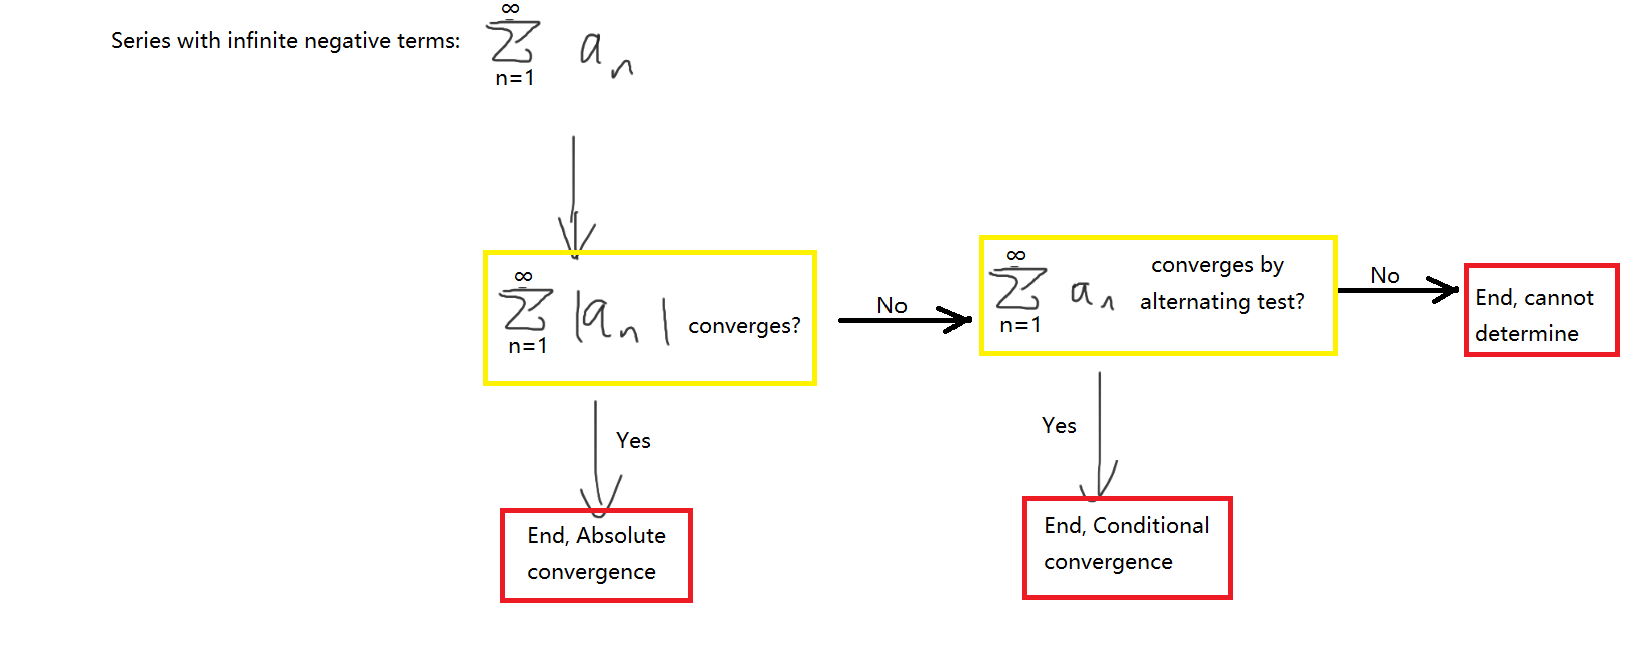
\includegraphics[width=1\textwidth]{program2.png}

Test we consider for proving convergence:
\begin{enumerate}
	\item The integral test
	\item p-test
	\item Comparison test
	\item Limit comparison test
	\item Check the absolute convergence of the series
	\item Ratio Test
	\item Alternating Series Test
\end{enumerate}

Test we consider for proving divergence:
\begin{enumerate}
	\item The integral test
	\item p-test
	\item Comparison test
	\item Limit comparison test
	\item Ratio Test
	\item Check $\lim_{n \to \infty} \neq 0$ or $\lim_{n \to \infty}$ does not exist.
\end{enumerate}

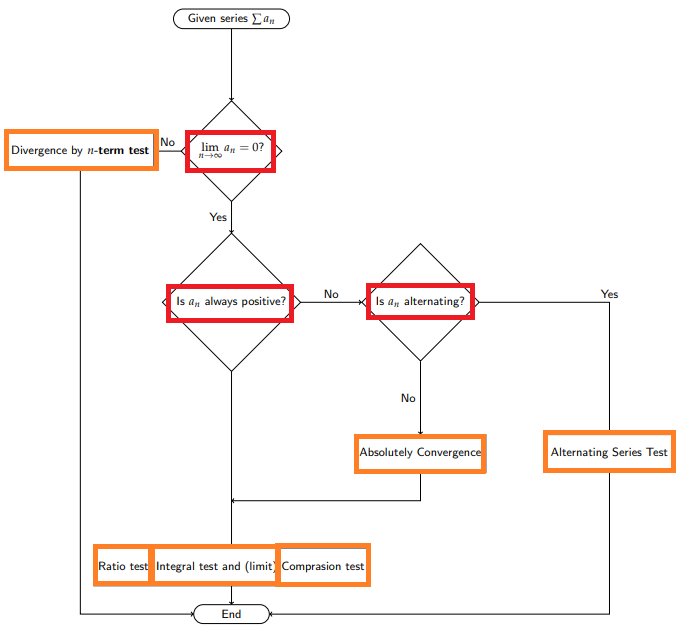
\includegraphics[width=1\textwidth]{program.png}


\subsection{Geometric Series}
There is a special series that we learn about, which is the Geometric Series, notice that the formula on the right hand side is what we called closed form. 
A finite geometric series has the form
\[a + ax + ax^2 + \cdots + ax^{n−2} + ax^{n−1}=\frac{a(1-x^n)}{1-x}\text{ For } x \neq 1\]
An infinite geometric series has the form
\[a + ax + ax^2 + \cdots + ax^{n−2} + ax^{n−1}+ax^n +\cdots=\frac{a}{1-x}\text{ For } |x| < 1\]

\newpage

\subsection{Power Series}
\begin{definition}
	A power series about $x = a$ is a sum of constants times powers of $(x - a)$: \\
	$C_0 + C_1(x - a) + C_2(x - a)^2 + \ldots + C_n(x - a)^n + \ldots =	\sum_{n
	=0}^{\infty}	C_n(x - a)^n$.
\end{definition}

If we fix a specific value of $x$, we can just consider plugging x with the value we have, and convergence here makes sense.

\begin{definition}
For a fixed value of $x$, if this sequence of partial sums converges to a limit $L$, that is, if
$\lim_{n \to \infty}S_n(x) = L$, then we say that the power series converges to $L$ for this value of $x$.
\end{definition}

Based on the discussion we will see that, The interval of convergence for a power series is usually centered at a point $x=a$, and extends the same length to both side, thus we denote this length as radius of convergence.\\

Moreover, each power series falls into one of the three following cases, characterized by its radius of convergence, $R$.
\begin{itemize}
\item The series converges only for $x = a$; the radius of convergence is defined to be $R = 0$.
\item The series converges for all values of $x$; the radius of convergence is defined to be
$R = \infty$.
\item There is a positive number $R$, called the radius of convergence, such that the series
converges for $|x - a| < R$ and diverges for $|x - a| > R$. 
\end{itemize}
The interval of convergence is the interval between $a - R$ and $a + R$, including any
endpoint where the series converges.


\end{document} 